\chapter{Theoretical Background}
\label{chap:theoretical-background}

This chapter establishes the theoretical foundation necessary for understanding the design and implementation of the \ac{VMAP} database system. It begins with an overview of automotive electronic control systems and parameter management, explaining the fundamental concepts that drive the requirements for the \ac{VMAP} system. The chapter then explores database management systems and design methodologies relevant to the implementation. Finally, it discusses foundational concepts in access control and version management that underpin the system architecture.

\section{Automotive Electronic Control Systems}
\label{sec:automotive-electronic-systems}

Modern commercial vehicles represent sophisticated cyber-physical systems where software controls virtually every aspect of vehicle operation. The complexity of these systems has grown exponentially over recent decades, with contemporary trucks containing dozens of interconnected \acp{ECU} working in concert to ensure optimal performance, efficiency, and safety \cite{staron2021automotive}. Understanding the structure and organization of these systems is essential for designing an effective parameter management solution.

\subsection{\ac{ECU} Hierarchy and Parameter Organization}
\label{subsec:ecu-hierarchy}

Automotive electronic systems follow a hierarchical organization that structures parameters into logical groupings reflecting the actual architecture of vehicle electronic systems. This hierarchy is not merely organizational but represents the fundamental structure of automotive software development, where components are modularized for maintainability, reusability, and functional separation \cite{pretschner2007software}.

\begin{figure}[ht]
    \centering
    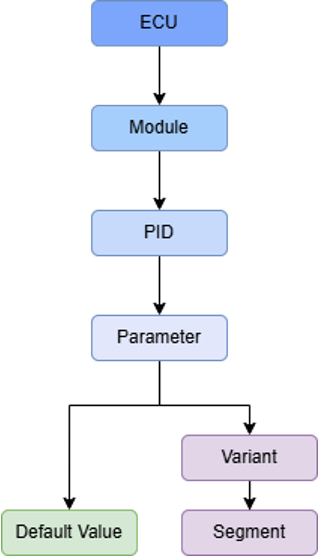
\includegraphics[height=0.4\textheight]{figures/ecu_hierarchy.png}
    \caption{Hierarchical Organization of Automotive Electronic Systems}
    \label{fig:ecu-hierarchy}
\end{figure}

At the highest level, \acp{ECU} represent distinct hardware components controlling specific vehicle functions such as engine management, transmission control, or brake systems. Each \ac{ECU} contains specialized software designed to manage particular aspects of vehicle operation, with the \ac{CPC} serving as a central control unit for critical powertrain functions \cite{kiencke2000automotive}. Within each \ac{ECU}, modules represent functional software units that implement specific capabilities such as cruise control, emission control, or diagnostic functions. This modular organization enables independent development and testing of different vehicle functions while maintaining clear interfaces between components.

Each module contains \acp{PID} that group related parameters according to their functional purpose. The \ac{PID} level provides a logical organization that reflects engineering workflows, where parameters are typically managed in functionally related groups rather than individually. Finally, individual parameters define specific configuration values that directly affect system behavior, ranging from simple scalar values to complex multi-dimensional lookup tables that define sophisticated control strategies \cite{staron2021autosar}.

Parameters themselves exhibit significant complexity beyond simple configuration values. Automotive control systems frequently employ parameters representing lookup tables, characteristic curves, and multi-dimensional maps that define control strategies for various operating conditions. For instance, an engine timing parameter might be represented as a three-dimensional array where engine speed, load, and temperature serve as independent variables determining the optimal ignition timing angle. This complexity in parameter structure creates specific requirements for database systems designed to manage automotive parameter data.

The hierarchical structure shown in Figure \ref{fig:ecu-hierarchy} illustrates how parameters can follow two distinct paths for value determination. Parameters may use their default values as defined in the baseline configuration, or they may be customized through variants that specify modified values for particular vehicle configurations or operating conditions. This dual-path approach enables efficient parameter management by storing only modifications rather than complete parameter sets for each vehicle variant.

\subsection{Parameter Variants and Customization}
\label{subsec:parameter-variants}

The automotive industry faces the challenge of supporting multiple parameter configurations for different vehicle variants, regional requirements, and operating conditions. Rather than maintaining separate complete parameter sets for each configuration, which would lead to significant redundancy and maintenance complexity, automotive systems implement a variant mechanism that allows selective overriding of parameter values based on specific conditions \cite{broy2006challenges}.

This variant approach operates on the principle that most parameters retain their default values across different vehicle configurations, with only a subset requiring modification for specific applications. Each parameter maintains a default value defined in the baseline configuration, which serves as the fallback value when no variant-specific override exists. Variants are created to represent specific vehicle configurations, market requirements, or operating conditions, with segments defining the actual modified parameter values within these variants. When no segment exists for a particular parameter within an applicable variant, the system automatically uses the default value, ensuring complete parameter coverage while minimizing storage requirements.

The variant selection process relies on code rules, which are boolean expressions that determine when a variant applies based on vehicle configuration codes. These expressions can represent simple conditions such as engine type selection or complex combinations involving multiple vehicle attributes such as transmission type, emission standard, and market destination. The code rule evaluation process occurs during parameter file generation, where the system determines which variants apply to a specific vehicle configuration and resolves the effective parameter values accordingly.

This approach creates specific requirements for database systems managing automotive parameters. The system must efficiently store and retrieve variant definitions while maintaining the complex relationships between parameters, variants, and segments. Additionally, the parameter resolution process must correctly apply variants based on vehicle configuration codes, ensuring that appropriate parameter values are selected for each specific vehicle configuration while maintaining performance for large parameter sets.

\subsection{Release and Phase Management}
\label{subsec:release-phase-management}

Automotive software development follows a structured release process with well-defined phases representing increasing levels of maturity and stability. This process reflects the engineering rigor required for safety-critical automotive systems, where parameter configurations must undergo systematic validation before implementation in production vehicles \cite{broy2006challenges}.

\begin{figure}[ht]
    \centering
    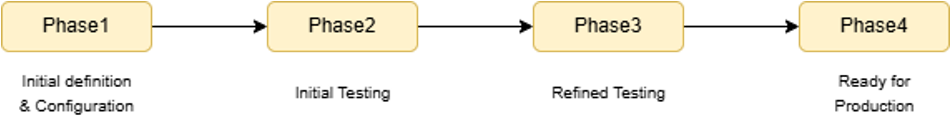
\includegraphics[width=0.85\textwidth]{figures/release_cycle.png}
    \caption{Automotive Parameter Release Cycle}
    \label{fig:release-cycle}
\end{figure}

The typical release cycle consists of bi-annual releases that align with automotive development schedules and market introduction timelines. Each release progresses through four sequential phases that represent distinct stages in the parameter development lifecycle. The Phase1 involves initial parameter definition and configuration, where new parameters are introduced and baseline configurations are established. Phase2 focuses on initial testing and refinement, where parameters undergo preliminary validation and adjustment based on early testing feedback. Phase3 continues the refinement process with more extensive testing, while Phase4 represents the completed configuration ready for production release.

Figure \ref{fig:release-cycle} illustrates the linear progression through these phases, with each phase building upon the work completed in the previous phase. This sequential structure ensures that parameter configurations mature systematically, with increasing levels of validation at each stage. The process accommodates the reality that different \acp{ECU} may progress through phases at different rates based on their development schedules, testing requirements, and dependency relationships with other vehicle systems.

Phase transitions represent critical points in the development process where parameter configurations are copied forward to establish a new baseline for continued development. This copying mechanism preserves the integrity of completed phases while enabling continued development in subsequent phases. Changes made in earlier phases should typically propagate to later phases unless explicitly overridden, creating requirements for change management and propagation mechanisms within the parameter management system.

The phase-based development process also includes mechanisms for freezing phases at specific development milestones. When a phase is frozen, its parameter configuration becomes read-only, creating a stable reference point for documentation, testing, and compliance activities. This freezing capability is essential for maintaining configuration control in regulated automotive development environments, where stable reference configurations must be preserved for audit and traceability purposes \cite{staron2021automotive}.

\section{Database Management Systems}
\label{sec:database-management-systems}

Database management systems provide the technological foundation for structured information storage, organization, and retrieval. They implement sophisticated mechanisms for ensuring data integrity, security, and concurrent access while supporting the complex queries and transactions required by modern applications \cite{sciore2009database}. For automotive parameter management, the selection and implementation of an appropriate database approach is critical for meeting the performance, reliability, and scalability requirements of engineering workflows.

\subsection{Relational Database Fundamentals}
\label{subsec:relational-database-fundamentals}

Relational database management systems organize data into structured tables composed of rows and columns, implementing the relational model proposed by E.F. Codd in 1970 \cite{codd1970relational}. The relational model establishes a mathematical foundation for representing data as relations with well-defined operations for data manipulation, providing a theoretically sound basis for database system implementation.

\begin{figure}[ht]
    \centering
    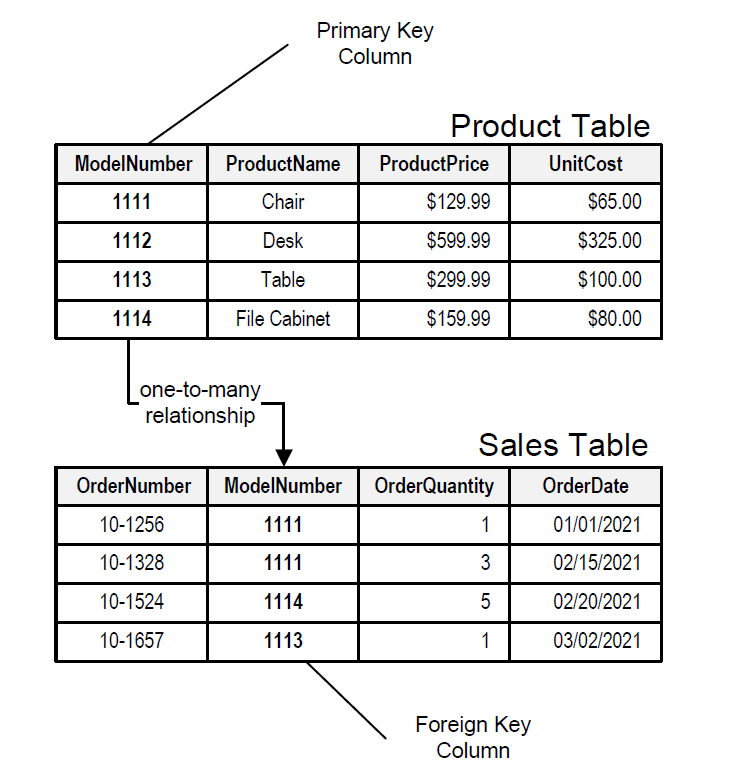
\includegraphics[width=0.85\textwidth]{figures/relational_schema.png}
    \caption{Example of a Relational Schema \cite{noah2024relational}}
    \label{fig:relational-schema}
\end{figure}

The relational model's strength lies in its systematic approach to data organization and integrity enforcement. Tables adhere to predefined schemas that specify structure, data types, and constraints applicable to the stored data. Each table includes a primary key that uniquely identifies each row, while foreign keys establish relationships between tables, implementing referential integrity that ensures consistency across related data. This structured approach enables complex queries across multiple related entities while maintaining data consistency through constraint enforcement.

Relational databases adhere to ACID properties that ensure reliable transaction processing in multi-user environments. Atomicity guarantees that transactions are treated as indivisible units that either complete entirely or have no effect, preventing partial updates that could leave the database in an inconsistent state. Consistency ensures that transactions transform the database from one valid state to another, maintaining all defined integrity constraints. Isolation prevents interference between concurrent transactions, enabling multiple users to work with the database simultaneously without conflicts. Durability ensures that committed transactions persist permanently, even in the event of system failures \cite{sciore2009database}.

For automotive parameter management, ACID compliance provides essential guarantees for data integrity and consistency. Parameter configurations directly affect vehicle behavior and safety, making the strong consistency guarantees of relational databases crucial for maintaining reliable parameter data. The hierarchical structure of automotive parameter systems, with well-defined relationships between \acp{ECU}, modules, \acp{PID}, and parameters, aligns naturally with the relational model's representation of structured data and entity relationships.

\subsection{Alternative Database Approaches}
\label{subsec:alternative-database-approaches}

Non-relational database systems, commonly referred to as \ac{NoSQL} databases, have emerged as alternatives to the relational model for specific application domains \cite{meier2019sql}. These systems typically prioritize scalability, flexibility, or performance characteristics over the strong consistency guarantees provided by relational databases \cite{brewer2000towards}.

\begin{figure}[ht]
    \centering
    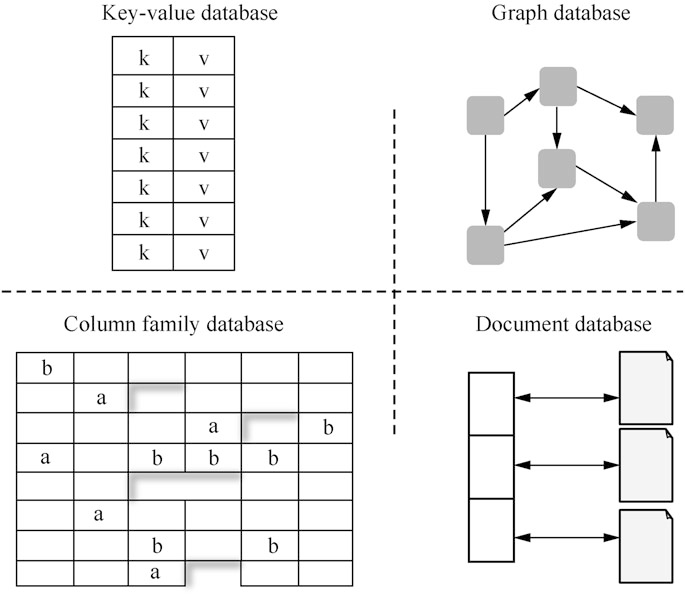
\includegraphics[width=0.85\textwidth]{figures/nosql_types.png}
    \caption{Major Types of NoSQL Databases \cite{gaussdbdatabase}}
    \label{fig:nosql-types}
\end{figure}

NoSQL databases can be categorized into several distinct types based on their data models and storage approaches \cite{meier2019sql}. Document databases store semi-structured data as documents, typically in JSON or XML formats, providing schema flexibility while maintaining query capabilities. Key-value stores offer simple key-based data access with high performance for specific access patterns. Column-family databases organize data in column-oriented structures that can efficiently handle sparse data and analytical workloads. Graph databases represent data as networks of interconnected nodes and relationships, excelling at representing and querying complex relationship structures.

Many NoSQL systems implement the BASE principle (Basically Available, Soft state, Eventually consistent) rather than ACID properties, prioritizing availability and partition tolerance over immediate consistency. This approach enables horizontal scaling across distributed systems but introduces complexity in managing data consistency and transaction semantics \cite{kleppmann2017conflict}.

While NoSQL databases excel in specific domains such as high-volume web applications, real-time analytics, and content management systems, they present challenges for applications requiring complex transactions, strict data integrity, or sophisticated queries across related entities \cite{meier2019sql}. For automotive parameter management, these limitations generally make NoSQL systems less suitable than relational databases, particularly given the critical importance of data consistency and the complex relational structure of automotive parameter data.

\section{Database Design Methodologies}
\label{sec:database-design-methodologies}

Database design methodologies provide systematic approaches for translating real-world information requirements into efficient, reliable database implementations. These methodologies ensure that database systems effectively support user needs while maintaining data integrity, performance, and maintainability \cite{chen1976entity}. This section explores the fundamental design approaches that form the theoretical foundation for database system development.

\subsection{Conceptual Modeling with Entity-Relationship Diagrams}
\label{subsec:conceptual-modeling}

Entity-relationship modeling provides a conceptual framework for representing the data structure needed to support identified system requirements. Introduced by Peter Chen in 1976, \ac{ER} modeling has become the predominant approach for conceptual database design due to its intuitive representation of real-world entities and their relationships \cite{chen1976entity}.

\begin{figure}[ht]
    \centering
    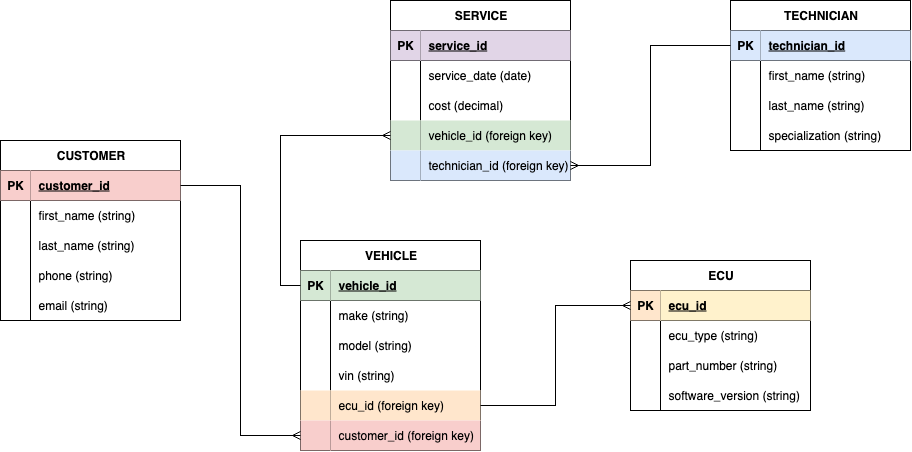
\includegraphics[width=0.95\textwidth]{figures/er_diagram.png}
    \caption{Entity-Relationship Diagram for an Automotive Service Center Database}
    \label{fig:er-diagram}
\end{figure}

The \ac{ER} model identifies three fundamental components that describe the structure of information systems. Entities represent the objects or concepts about which information needs to be stored, such as customers, products, or in an automotive context, vehicles, \acp{ECU}, or parameters. Attributes describe the specific properties or characteristics of each entity, such as names, identifiers, values, or descriptive information. Relationships describe the associations between entities, expressing how different objects in the system interact or relate to one another.

Figure \ref{fig:er-diagram} illustrates these concepts in a practical context, showing how entities, attributes, and relationships combine to represent a comprehensive information structure. The diagram demonstrates the use of primary keys for unique entity identification, foreign keys for relationship implementation, and the various types of relationships that can exist between entities in a complex system.

\ac{ER} modeling is particularly valuable for complex domains like automotive systems because it provides a visual representation that stakeholders can understand while being precise enough to guide database implementation. Chen explains that the \ac{ER} model adopts a natural view of the world consisting of entities and relationships, making it an intuitive approach for modeling real-world systems while maintaining the precision required for technical implementation \cite{chen1976entity}.

\subsection{Data Normalization Principles}
\label{subsec:data-normalization}

Database normalization provides a systematic process for organizing data to minimize redundancy and prevent update anomalies. Developed by E.F. Codd as part of the relational model, normalization proceeds through several normal forms, each addressing specific types of data inconsistencies and structural problems \cite{codd1970relational}.

The normalization process begins with First Normal Form, which requires that each cell in a table contains only atomic values rather than lists or repeating groups. This ensures that data elements are indivisible and can be manipulated consistently using relational operations. Second Normal Form builds upon this foundation by requiring that all non-key attributes depend functionally on the entire primary key, preventing partial dependencies that can lead to update anomalies. Third Normal Form further refines the structure by eliminating transitive dependencies, ensuring that non-key attributes depend only on the primary key rather than on other non-key attributes \cite{sciore2009database}.

For most practical applications, achieving Third Normal Form provides an appropriate balance between data integrity and system performance. As explained by Simon, Third Normal Form is considered adequate for most practical purposes, with further normalization typically performed only when specific data integrity requirements demand additional refinement \cite{simongetting}.

In automotive parameter management, normalization helps organize complex data about \acp{ECU}, modules, and parameters into a structure that maintains consistency while supporting efficient access. Proper normalization ensures that parameter definition changes need to be recorded in only one location, eliminating the risk of inconsistent values across the database while supporting the complex relationships inherent in automotive electronic systems.

\section{Access Control and Security Fundamentals}
\label{sec:access-control-security}

Database systems frequently contain sensitive information that requires controlled access based on user roles and responsibilities. Access control mechanisms provide systematic approaches to managing permissions while maintaining security and supporting organizational workflows \cite{sandhu1998role}. This section examines the fundamental concepts that underpin access control implementation in database systems.

\subsection{Role-Based Access Control Principles}
\label{subsec:rbac-principles}

Role-Based Access Control represents a systematic approach to managing user permissions by associating permissions with roles rather than individual users. Introduced by David Ferraiolo and Richard Kuhn, \ac{RBAC} has become the predominant model for access control in enterprise systems due to its balance of security effectiveness and administrative simplicity \cite{sandhu1998role}.

The fundamental concept of \ac{RBAC} involves organizing permissions around roles that correspond to job functions within an organization. Rather than granting permissions directly to individual users, the system defines roles such as administrator, engineer, or analyst, with each role receiving a specific set of permissions appropriate to its responsibilities. Users are then assigned to appropriate roles, inheriting the permissions associated with those roles.

This approach provides significant advantages over direct permission assignment. Administrative complexity is reduced by managing permissions at the role level rather than for individual users, simplifying the process of granting appropriate access to new users or modifying access when job responsibilities change. Security is enhanced through implementation of the principle of least privilege, ensuring that users receive only the permissions necessary for their specific responsibilities. The role abstraction also provides a clear mapping between organizational responsibilities and system permissions, making access control policies easier to understand and audit \cite{ferraiolo2011policy}.

The theoretical foundation of \ac{RBAC} includes several key components that work together to provide flexible access control. Users represent individuals who require access to system resources. Roles represent collections of permissions that correspond to specific job functions or responsibilities within the organization. Permissions define specific operations that can be performed on particular resources or data elements. Sessions provide temporary bindings between users and their assigned roles, enabling dynamic activation of different permission sets based on current activities \cite{sandhu1997arbac97}.

\subsection{Database Security Implementation}
\label{subsec:database-security}

Modern database management systems provide various mechanisms for implementing access control policies, ranging from basic user authentication to sophisticated role-based permission systems. These mechanisms operate at multiple levels within the database system, from table-level access control to row-level security policies that can restrict access based on data content \cite{shaik2020postgresql}.

Database-level security typically begins with user authentication, where the system verifies user identity before granting access to database resources. Once authenticated, authorization mechanisms determine which operations the user can perform on specific database objects such as tables, views, or stored procedures. Most enterprise database systems support role-based approaches where users can be assigned to roles that define their permitted operations, implementing \ac{RBAC} principles at the database level.

However, database-level \ac{RBAC} implementations typically focus on controlling access to database objects rather than providing application-level access control that considers domain-specific entities and operations. For complex applications like automotive parameter management, database-level security must be complemented with application-level access control logic that maps domain-specific concepts to database operations while maintaining the security guarantees provided by the underlying database system \cite{sciore2009database}.

\section{Version Control and Temporal Data Concepts}
\label{sec:version-control-temporal}

Many applications require tracking how data changes over time, maintaining historical states, and supporting queries based on temporal relationships. This section examines the fundamental concepts that underpin version control and temporal data management in database systems.

\subsection{Version Control Fundamentals}
\label{subsec:version-control-fundamentals}

Version control for database content addresses the challenge of tracking changes to structured data with complex relationships and constraints. Unlike traditional source code version control systems that manage text files, database version control must maintain referential integrity while preserving historical states and supporting evolution through distinct development stages \cite{tichy1985rcs}.

Several fundamental approaches exist for implementing version control in database systems. The snapshot approach captures complete database states at specific points in time, providing straightforward retrieval of historical states but potentially consuming significant storage resources. The delta-based approach records only modifications to database content, reducing storage requirements but requiring reconstruction of historical states through the application of change records. The temporal approach extends traditional database structures with time dimensions, enabling direct querying of historical states through time-based predicates \cite{bhattacherjee2015principles}.

The selection of an appropriate version control approach depends on specific application requirements, particularly the frequency of historical data access, the complexity of change patterns, and the performance requirements for both current and historical data operations. Bhattacherjee et al. note that domain-specific versioning approaches often provide better performance and usability than generic temporal database techniques when tailored to specific application requirements \cite{bhattacherjee2015principles}.

\subsection{Temporal Database Concepts}
\label{subsec:temporal-database-concepts}

Temporal database concepts provide theoretical foundations for managing time-varying data in database systems. Unlike traditional databases that store only current states, temporal databases maintain historical information and support queries based on time relationships \cite{snodgrass1999developing}.

\begin{figure}[ht]
    \centering
    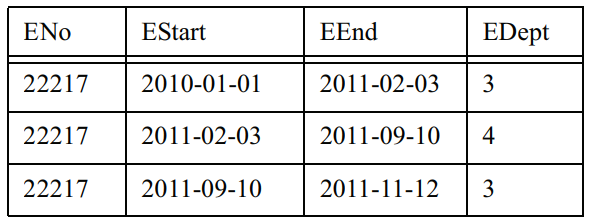
\includegraphics[width=0.8\textwidth]{figures/temporal_database.png}
    \caption{Temporal Table Tracking Employee Department History \cite{kulkarni2012temporal}}
    \label{fig:temporal-database}
\end{figure}

Temporal databases typically support two fundamental time dimensions. Valid time represents when facts are true in the modeled reality, independent of when they are recorded in the database. Transaction time represents when facts are recorded in the database system, independent of when they become true in reality. Databases that support both dimensions simultaneously are known as bi-temporal databases, providing comprehensive temporal functionality for applications requiring both historical accuracy and change auditability \cite{kulkarni2012temporal}.

Figure \ref{fig:temporal-database} illustrates a practical implementation of temporal concepts, showing how historical information can be maintained through time-based table structures. The example demonstrates how temporal tables can track the complete history of entity state changes without overwriting previous records, enabling historical queries and analysis.

Temporal database implementations often employ specialized table structures that extend traditional schemas with timestamp columns defining validity periods for each record. This approach enables systematic tracking and querying of historical data without requiring application-level version management, providing a foundation for maintaining comprehensive audit trails and supporting historical analysis requirements \cite{salzberg1999comparison}.
